\documentclass[a4paper]{article}
\usepackage[12pt]{extsizes}
\usepackage[utf8]{inputenc}
\usepackage[russian]{babel}
\usepackage{setspace}
\usepackage{amsmath}
\usepackage[left=10mm, top=15mm, right=10mm, bottom=15mm, nohead, footskip=10mm]{geometry} 
\usepackage{wrapfig}
\usepackage[pdftex]{graphicx}
\usepackage{indentfirst}
\graphicspath{{pictures/}}
\DeclareGraphicsExtensions{.eps,.pdf,.png,.jpg}
\begin{document}
\setcounter{page}{0} 
\begin{titlepage}
\begin{center}
\largel{\textbf{МОСКОВСКИЙ ГОСУДАРСТВЕННЫЙ УНИВЕРСИТЕТ\\ИМЕНИ М.В. ЛОМОНОСОВА}}\\
\hfill\break
\normalsize{ФИЗИЧЕСКИЙ ФАКУЛЬТЕТ}\\
 \hfill\break
\normalsize{ГОСУДАРСТВЕННЫЙ АСТРОНОМИЧЕСКИЙ ИНСТИТУТ ИМЕНИ П.К. ШТЕРНБЕРГА}\\
\hfill\break
\hfill\break
\hfill\break
\hfill\break
\hfill\break
\hfill\break
\hfill\break
\hfill\break
\largel{\textbf{ОПРЕДЕЛЕНИЕ ЭФФЕКТИВНОСТИ ИНФРАКТРАСНОЙ КАМЕРЫ\\ПРИ РАБОТЕ В СПЕКТРОСКОПИЧЕСКОМ РЕЖИМЕ}\\
\hfill\break
\normalsize{(И.А. ОРЛОВ, Н.А. МИТИЧКИН)}\\
\end{center}
\hfill\break
\hfill\break
\hfill\break
\hfill\break
\hfill\break
\hfill\break
\hfill\break
\hfill\break
\hfill\break
\hfill\break
\hfill\break
\hfill\break
\hfill\break
\hfill\break
\hfill\break
\hfill\break 
\hfill\break
\hfill\break
\hfill\break
\hfill\break
\hfill\break
\hfill\break
\hfill\break
\hfill\break
\hfill\break
\hfill\break
\hfill\break
\begin{center}
Кавказская горная обсерватория ГАИШ МГУ имени М.В. Ломоносова, июль 2018 г.
\end{center}
\thispagestyle{empty}
\end{titlepage}
\newpage
\tableofcontents
\newpage
\section{Введение}
\begin{wrapfigure}[12]{r}{0.40\linewidth} 
\vspace{-4ex}
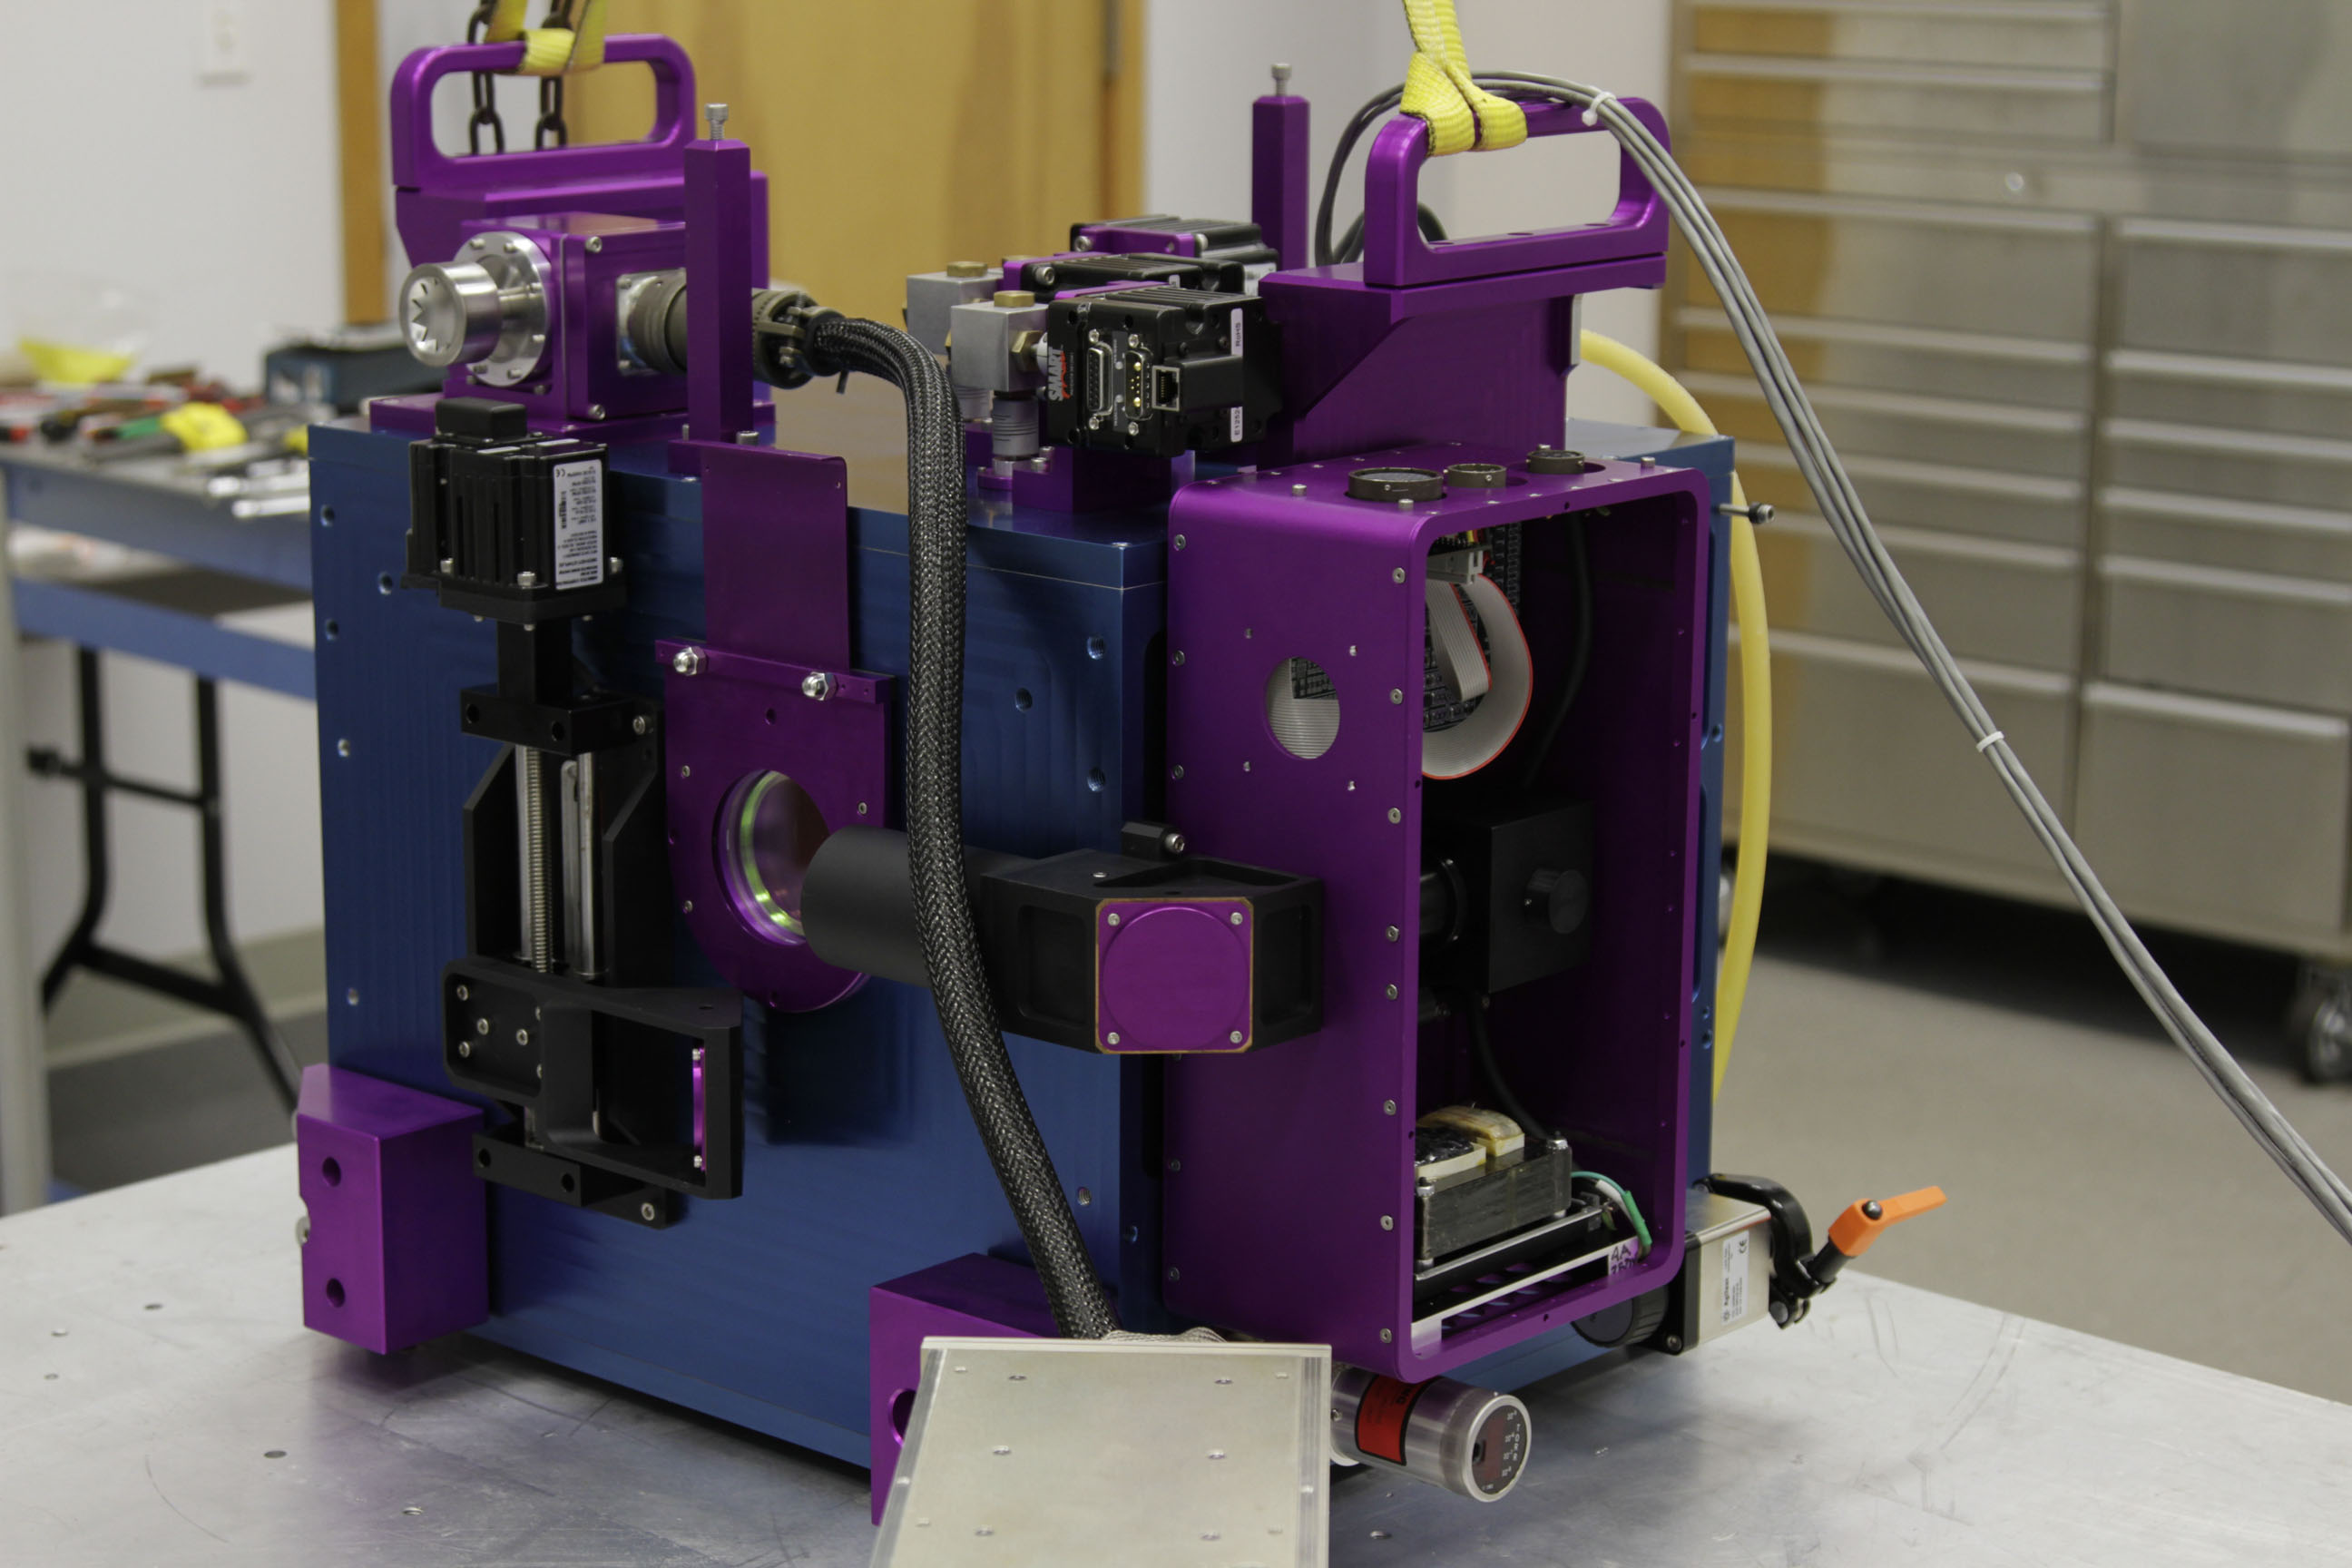
\includegraphics[width=\linewidth]{11}
\caption{Внешний вид устройства ASTRONIRCAM.}
\label{fig:1}
\end{wrapfigure}
& &Основной задачей данной работы является определние эффективности инфракрасной камеры прибора ASTRONIRCAM при работоте в спетроскопическом режиме.

ASTRONIRCAM - это криогенно-охлаждае-мый щелевой спектрограф на спектральную область 1-2.5 мкм, установленный в фокусе Нэсмита\footnote{Система Нэсмита - это трехзеркальная модификация системы Кассегрена, в которой внутри трубы телескопа между главным и вторичным зеркалами установлено диагональное зеркало для отбрасывания изображения вбок. Таким образом, фокус телескопа, называемый фокусом Несмита, находится сбоку трубы. Такая оптическая схема позволяет нагружать телескоп громоздким наблюдательным оборудованием, без разбалансирования трубы.} 2.5-м телескопа Кавказской горной обсерватории ГАИШ МГУ имени М.В. Ломоносова. При работе в спектроскопическом режиме прибор позволяет получать спектры протяжённых и точечных астрономических объектов с разрешающей силой $R = \dfrac{\lambda}{\delta\lambda}\leq 1200$.

Подробнее про принцип и особенности работы прибора ASTRONIRCAM можно прочесть в \cite{Sulsky1994}.

\hfill\break

\section{Наблюдения}
Одним из первых этапов выполнения задачи являлось получение спектров исследуемой звезды HIP85382 звёздного класса A0V. Наблюдения проводились с использованием последовательно двух щелей STIT6 и SLIT7 и фотометрических фильтров: Y, J, H и K. Результаты наблюдений представлены на Рис. 2, Рис. 3 и Рис








\hfill\break

\begin{thebibliography}{3}
\bibitem{Sulsky1994}
А. Э. Наджип, А. М. Татарников, Д. У. Туми, Н. И. Шатский, А. М. Черепащук, С. А. Ламзин, А. А. Белинский,  ASTRONIRCAM - инфракрасная камера-спектрограф 2.5-м телескопа КГО ГАИШ, (16 июня 2017 г.).
\end{thebibliography}
\end{document}


\end{document}  % КОНЕЦ ДОКУМЕНТА !